\documentclass[a4paper,14pt]{report}
\usepackage[T2A]{fontenc}
\usepackage[utf8]{inputenc}
\usepackage[english,russian]{babel}
\usepackage{listings}
\usepackage{geometry}
\usepackage{amssymb}
\usepackage{amsmath}
\usepackage[14pt]{extsizes}
\geometry{left=2cm}
\geometry{right=1.5cm}
\geometry{top=1cm}
\geometry{bottom=2cm}
\pagestyle{plain}
\usepackage{pgfplots}
\usepackage{filecontents}
\usepackage{graphicx}
\usepackage{indentfirst}
\DeclareGraphicsExtensions{.png}
\graphicspath{{images/}}
\usetikzlibrary{datavisualization}
\usetikzlibrary{datavisualization.formats.functions}

\usepackage{tocloft}

\renewcommand\cftchapdotsep{\cftdot}
\renewcommand\cftsecdotsep{\cftdot}
\renewcommand{\cftchapleader}{\cftdotfill{\cftchapdotsep}}

\begin{filecontents}{insBest.dat}
0 0.0000008500
100 0.0000017900
200 0.0000025700
300 0.0000041400
400 0.0000039200
500 0.0000047700
600 0.0000054600
700 0.0000077900
800 0.0000067900
900 0.0000052600
1000 0.0000050100
%1100 0.0000048600
%1200 0.0000054700
%1300 0.0000057900
%1400 0.0000061300
%1500 0.0000065600
%1600 0.0000070000
%1700 0.0000073900
%1800 0.0000078700
%1900 0.0000081300
%2000 0.0000087400
\end{filecontents}

\begin{filecontents}{insAvg.dat}
	0 0.0000008400
	100 0.0000019100
	200 0.0000034400
	300 0.0000050500
	400 0.0000062100
	500 0.0000081400
	600 0.0000107300
	700 0.0000141300
	800 0.0000148200
	900 0.0000137500
	1000 0.0000150600
	%1100 0.0000134500
	%1200 0.0000152500
	%1300 0.0000173200
	%1400 0.0000197300
	%1500 0.0000214900
	%1600 0.0000238900
	%1700 0.0000269700
	%1800 0.0000294500
	%1900 0.0000325000
	%2000 0.0000371100
\end{filecontents}

\begin{filecontents}{insWorst.dat}
	0 0.0000008400
	100 0.0000020700
	200 0.0000038500
	300 0.0000072300
	400 0.0000082200
	500 0.0000113200
	600 0.0000148100
	700 0.0000203600
	800 0.0000233000
	900 0.0000217700
	1000 0.0000212200
	%1100 0.0000210100
	%1200 0.0000245900
	%1300 0.0000281000
	%1400 0.0000325900
	%1500 0.0000363700
	%1600 0.0000427100
	%1700 0.0000456200
	%1800 0.0000507100
	%1900 0.0000558400
	%2000 0.0000628500
\end{filecontents}

\begin{filecontents}{bubbleBest.dat}
	0 0.0000007100
	100 0.0000011200
	200 0.0000018900
	300 0.0000012100
	400 0.0000015000
	500 0.0000017300
	600 0.0000021900
	700 0.0000022500
	800 0.0000025300
	900 0.0000028100
	1000 0.0000030700
	%1100 0.0000033600
	%1200 0.0000036200
	%1300 0.0000038400
	%1400 0.0000041000
	%1500 0.0000044200
	%1600 0.0000046600
	%1700 0.0000050200
	%1800 0.0000052200
	%1900 0.0000054900
	%2000 0.0000057500
\end{filecontents}

\begin{filecontents}{bubbleAvg.dat}
	0 0.0000007500
	100 0.0000021600
	200 0.0000051100
	300 0.0000091400
	400 0.0000084500
	500 0.0000130200
	600 0.0000183800
	700 0.0000243800
	800 0.0000327400
	900 0.0000398100
	1000 0.0000490000
	%1100 0.0000599200
	%1200 0.0000703000
	%1300 0.0000834500
	%1400 0.0000963000
	%1500 0.0001102700
	%1600 0.0001249100
	%1700 0.0001436100
	%1800 0.0001595000
	%1900 0.0001787800
	%2000 0.0001997900
\end{filecontents}

\begin{filecontents}{bubbleWorst.dat}
	0 0.0000015900
	100 0.0000056000
	200 0.0000131700
	300 0.0000202500
	400 0.0000291200
	500 0.0000312000
	600 0.0000339300
	700 0.0000342900
	800 0.0000531000
	900 0.0000522700
	1000 0.0000642600
	%1100 0.0000786700
	%1200 0.0000928900
	%1300 0.0001071700
	%1400 0.0001248600
	%1500 0.0001423100
	%1600 0.0001617600
	%1700 0.0001817900
	%1800 0.0002047900
	%1900 0.0002274200
	%2000 0.0002641400
\end{filecontents}


\begin{filecontents}{qsortBest.dat}
	0 0.0000007400
	100 0.0000235400
	200 0.0000585900
	300 0.0001266100
	400 0.0002221900
	500 0.0003416100
	600 0.0004876100
	700 0.0006598300
	800 0.0008609000
	900 0.0010870500
	1000 0.0013407200
	%1100 0.0016318000
	%1200 0.0019193800
	%1300 0.0022442900
	%1400 0.0026002100
	%1500 0.0029828500
	%1600 0.0033888600
	%1700 0.0038240200
	%1800 0.0042906300
	%1900 0.0047722800
	%2000 0.0052887500
\end{filecontents}

\begin{filecontents}{qsortAvg.dat}
	0 0.0000015100
	100 0.0000510600
	200 0.0001014800
	300 0.0001262500
	400 0.0002193100
	500 0.0003386100
	600 0.0004841400
	700 0.0006551700
	800 0.0008677500
	900 0.0010810000
	1000 0.0013233900
	%1100 0.0015982800
	%1200 0.0019036100
	%1300 0.0022248300
	%1400 0.0025790800
	%1500 0.0029560100
	%1600 0.0033742500
	%1700 0.0037914800
	%1800 0.0042506700
	%1900 0.0047277500
	%2000 0.0052338100
\end{filecontents}

\begin{filecontents}{qsortWorst.dat}
	0 0.0000018400
	100 0.0000225700
	200 0.0000584400
	300 0.0001269100
	400 0.0002199800
	500 0.0003397000
	600 0.0004850300
	700 0.0006568800
	800 0.0008539500
	900 0.0010768000
	1000 0.0013256300
	%1100 0.0016005700
	%1200 0.0019011700
	%1300 0.0022283400
	%1400 0.0025799000
	%1500 0.0029639100
	%1600 0.0033647900
	%1700 0.0037916400
	%1800 0.0042481700
	%1900 0.0047295700
	%2000 0.0052383800
\end{filecontents}

% Для листинга кода:
\lstset{ %
language=python,                 % выбор языка для подсветки
basicstyle=\small\sffamily, % размер и начертание шрифта для подсветки кода
numbers=left,               % где поставить нумерацию строк (слева\справа)
numberstyle=\tiny,           % размер шрифта для номеров строк
stepnumber=1,                   % размер шага между двумя номерами строк
numbersep=5pt,                % как далеко отстоят номера строк от подсвечиваемого кода
showspaces=false,            % показывать или нет пробелы специальными отступами
showstringspaces=false,      % показывать или нет пробелы в строках
showtabs=false,             % показывать или нет табуляцию в строках
frame=single,              % рисовать рамку вокруг кода
tabsize=4,                 % размер табуляции по умолчанию равен 2 пробелам
captionpos=t,              % позиция заголовка вверху [t] или внизу [b]
breaklines=true,           % автоматически переносить строки (да\нет)
breakatwhitespace=false, % переносить строки только если есть пробел
escapeinside={\#*}{*)}   % если нужно добавить комментарии в коде
}

% Для измененных титулов глав:
\usepackage{titlesec, blindtext, color} % подключаем нужные пакеты
\definecolor{gray75}{gray}{0.75} % определяем цвет
\newcommand{\hsp}{\hspace{20pt}} % длина линии в 20pt
% titleformat определяет стиль
\titleformat{\chapter}[hang]{\Huge\bfseries}{\thechapter\hsp\textcolor{gray75}{|}\hsp}{0pt}{\Huge\bfseries}



\begin{document}
\begin{titlepage}
	\centering
	{\scshape\LARGE МГТУ им. Баумана \par}
	\vspace{3cm}
	{\scshape\Large Лабораторная работа №3\par}
	\vspace{0.5cm}
	{\scshape\Large По курсу: "Анализ алгоритмов"\par}
	\vspace{1.5cm}
	{\huge\bfseries Трудоемкость сортировок\par}
	\vspace{2cm}
	\Large Работу выполнила: Овчинникова Анастасия, ИУ7-55Б\par
	\vspace{0.5cm}
	\LargeПреподаватели:  Волкова Л.Л., Строганов Ю.В.\par

	\vfill
	\large \textit {Москва, 2019} \par
\end{titlepage}

\tableofcontents

\newpage
\chapter*{Введение}
\addcontentsline{toc}{chapter}{Введение}

Целью данной работы является изучение алгоритмов сортировки массивов, сравнительный анализ времени работы алгоритмов и анализ их трудоемкости.

Задачи лабораторной работы:
\begin{enumerate}
	\item реализовать алгоритм сортировки вставками;
	\item реализовать алгоритм быстрой сортировки;
	\item реализовать алгоритм сортировки пузырьком с флагом;
	\item провести оценку трудоемкости алгоритмов сортировки вставками, быстрой сортировки и сортировки пузырьком с флагом;
	\item провести анализ времени работы алгоритмов размера от 100 до 2000 элементов.
\end{enumerate}


\chapter*{Аналитическая часть}
\addcontentsline{toc}{chapter}{Аналитическая часть}

Под сортировкой в программировании понимается такая перестановка предметов, при которой они располагаются в порядке возрастания или убывания. Д. Кнут в [4] выделяет слудующие наиболее важные области применения сортировки.
\begin{enumerate}
	\item Решение задачи группирования, когда нужно собрать вместе все элементы с одинаковыми значениями некоторого признака.
	\item Поиск общих элементов в двух или более массивах.
	\item Поиск информации по значениям ключей.
	\item Провести оценку трудоемкости алгоритмов сортировки вставками, быстрой сортировки и пузырьковой сортировки.
	\item Провести анализ времени работы алгоритмов размера от 100 до 1000 элементов.
\end{enumerate}

Исторически сложилось так, что на сортировку уходит больше компьютерного времени, чем на остальные задачи. Поэтому сортировка - самая изученная задача в теории вычислительных систем.
Известны десятки алгоритмов сортировки, большинство из которых имеют определенное преимущество над другими алгоритмами в определенных ситуациях.
Далее будут рассмотрены алгоритм сортировки вставкам, алгоритм быстрой сортировки и алгоритм сортировки пузырьком.

\section*{Описание алгоритмов}
\addcontentsline{toc}{section}{Описание алгоритмов}

\subsection*{Алгоритм сортировки вставками}
\addcontentsline{toc}{subsection}{Алгоритм сортировки вставками}

Основная идея сортировки вставками состоит в том, что при добавлении нового элемента в уже отсортированный список его стоит сразу вставлять в нужное место.
Сортировка вставками считает первый элемент любого списка отсортированным списком длины 1.
Двухэлементный отсортированный список создается добавлением второго элемента исходного списка в нужное место одноэлементного списка, содержащего первый элемент.
Теперь можно вставить третий элемент исходного списка в отсортированный двухэлементный список. Этот процесс повторяется до тех пор, пока всеэлементы исходного списка не окажутся в расширяющейся отсортированной части списка.

\subsection*{Алгоритм быстрой сортировки}
\addcontentsline{toc}{subsection}{Алгоритм быстрой вставками}

Быстрая сортировка является рекурсивным алгоритмом сортировки.
Быстрая сортировка выбирает элемент списка, называемый осевым, а затем переупорядочивает список таким образом, что все элементы, меньшие осевого, оказываются перед ним, а большие элементы - за ним. В каждой из частей списка элементы не упорядочиваются.
Если s — окончательное положение осевого элемента, то нам известно лишь, что все значения в позициях с первой по s — 1 меньше осевого, а значения с номерами от s + 1 до N больше осевого. Затем алгоритм быстрой сортировки вызывается рекурсивно на каждой из двух частей.
При вызове процедуры Quicksort на списке, состоящем из одного элемента, он ничего не делает, поскольку одноэлементный список уже отсортирован.

Функция для расщепления списка PivotList берет в качестве осевого элемента первый элемент списка и устанавливает указатель pivot в начало списка. Затем она проходит по списку, сравнивая осевой элемент с остальными элементами списка. Обнаружив элемент, меньший осевого, она увеличивает указатель PivotPoint, а затем переставляет элемент с новым номером PivotPoint и вновь найденный элемент. После того, как сравнение части списка с осевым элементом уже произведено, список оказывается разбит на четыре части. Первая часть состоит из первого осевого — элемента списка. Вторая часть начинается с положения first + 1,кончается в положении PivotPoint и состоит из всех просмотренныэлементов, оказавшихся меньше осевого. Третья часть начинается вположении PivotPoint+1 и заканчивается указателем параметра цикла index. Оставшаяся часть списка состоит из еще не просмотренных значений.

\subsection*{Алгоритм сортировки пузырьком с флагом}
\addcontentsline{toc}{subsection}{Алгоритм сортировки пузырьком с флагом}

Основной принцип сортировки пузырьком состоит в выталкивании маленьких значений на вершину списка в то время, как большие значения опускаются вниз. Алгоритм пузырьковой сортировки совершает несколько проходов по списку.
При каждом проходе происходит сравнение соседних элементов. Если порядок соседних элементов неправильный, то они меняются местами. Каждый проход начинается с начала списка.
Сперва сравниваются первый и второй элементы, затем второй и третий, потом третий и четвертый и так далее; элементы с неправильным порядком в паре переставляются.
При обнаружении на первом проходе наибольшего элемента списка он будет переставляться со всеми последующими элементами пока не дойдет до конца списка. Поэтому при втором проходе нет необходимости производить сравнение с последним элементом.
При втором проходе второй по величине элемент списка опустится во вторую позицию с конца.
При продолжении процесса на каждом проходе по крайней мере одно из следующих по величине значений встает на свое место.
При этом меньшие значения тоже собираются наверху. Если при каком-то проходе не произошло ни одной перестановки элементов, то все они стоят в нужном порядке, и исполнение алгоритмаможно прекратить.
Стоит заметить, что при каждом проходе ближе к своему месту продвигается сразу несколько элементов, хотя гарантированно занимает окончательное положение лишь один.


\subsection*{Модель вычислений}
\addcontentsline{toc}{subsection}{Модель вычислений}

Трудоемкость алгоритма измеряется в количестве операций, которые необходимо выполнить.

Введем модель вычислений, используемую при оценке трудоемкости алгоритмов.

\begin{enumerate}
	\item Базовые операции трудоемкости 1: +, -, *, /, =, ==, <=, >=, !=, >, <, +=, -=, |=, *=, проход по адресу.
	\item Трудоемкость цикла вычисляется по формуле $f = 2 + N(2 + f_{body})$, где $N$ - число повтрорений цикла, $f_{body}$ - трудоемкость тела цикла.
	\item Трудоемкость условного перехода равна 0, стоимость вычисления условия остается.
	\item Вызов метода объекта класса имеет трудоемкость 1.
	\item Объявление переменной/массива/структуры без определения имеет трудоемкость 0.\
	\item Условный оператор без условий внутри имеет трудоемкость 0.
	\item Логические операции имеют трудоемкость 1.
\end{enumerate}


\chapter*{Конструкторская часть}
\addcontentsline{toc}{chapter}{Конструкторская часть}

\section*{Требования к программе}
\addcontentsline{toc}{section}{Требования к программе}

Программа представляет собой консольное приложение с меню для выбора пользователем необходимого действия.
Меню содержит следующие пункты:
\begin{itemize}
	\item "1 - сортировка случайного масива с помощью алгоритма сортировки вставками";
	\item "2 - сортировка случайного масива с помощью алгоритма сортировки пузырьком";
	\item "3 - сортировка случайного масива с помощью алгоритма быстрой сортировки";
	\item "4 - временной анализ";
	\item "5 - тесты".
\end{itemize}

Для выбора соответствующих пунктов меню пользователь вводит соответствующую цифру (1-5). При вводе любого другого символа программа должна корректно завершаться. Для пунктов 1 - 3 программа просит пользователя ввести желаемую длину случайного массива. Затем она генерирует случайный массив указанной длины с помощью втроенной функции rand().

Далее в данном разделе будут рассмотрены схемы выбранных алгоритмов сортировки.

\section*{Схемы алгоритмов}
\addcontentsline{toc}{section}{Схемы алгоритмов}

Схема алгоритма сортировки вставками представлена на рисунке 1. Схема алгоритма пузырьковой сортировки представлена на рисунке 2. Схема алгоритма быстрой сортировки представлена на рисунке 3, а подпрограмма pivotList для разбиение массива, используемая в быстрой сортировке, представлена на рисунке 4.
В алгоритмах используется функция std::swap(T\& a, T\& b) из C++ библиотеки <utility>, которая меняет местами значения a и b.

\begin{figure}
\center{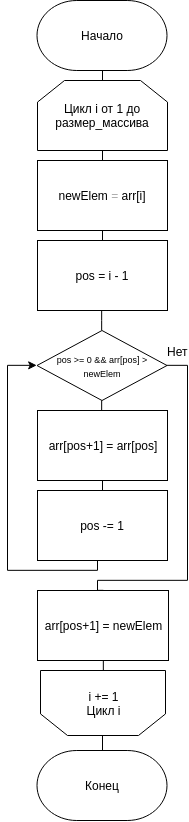
\includegraphics[height=20cm]{insertion_sort.png}}
\caption{Схема алгоритма сортировки вставками}
\label{fig:image}
\end{figure}

\begin{figure}
\center{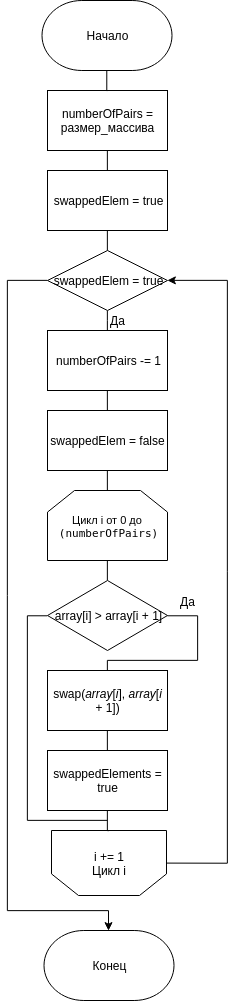
\includegraphics[height=20cm]{bubble_sort.png}}
\caption{Схема алгоритма пузырьковой сортировки}
\label{fig:image}
\end{figure}

\begin{figure}
\center{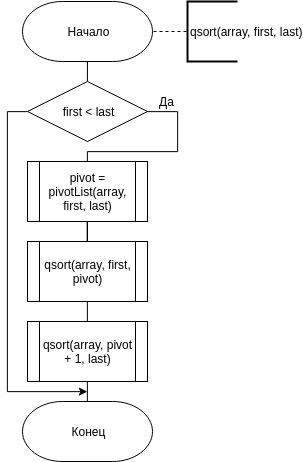
\includegraphics[height=15cm]{qsort.png}}
\caption{Схема алгоритма быстрой сортировки}
\label{fig:image}
\end{figure}

\begin{figure}
\center{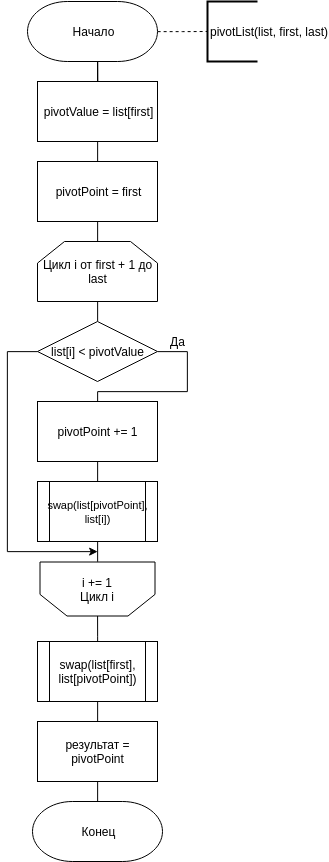
\includegraphics[height=20cm]{qsort_pivot.png}}
\caption{Схема подпрограммы pivotList}
\label{fig:image}
\end{figure}


\chapter*{Технологическая часть}
\addcontentsline{toc}{chapter}{Технологическая часть}

\section*{Выбор языка программирования}
\addcontentsline{toc}{section}{Выбор языка программирования}

В качестве языка программирования для реализации программы был выбран язык C++ и фреймворк Qt, потому что:
\begin{itemize}
	\item язык C++ имеет высокую вычислительную производительность;
	\item язык C++ поддерживает различные стили программирования;
	\item в Qt существует удобный инструмент для тестирования - QtTest - который позволяет собирать тесты в группы, собирать результаты выполнения тестов, а также уменьшить дублирование кода при схожих объектах тестирования.
\end{itemize}

Для замеров времени использовалась функция clock() модуля ctime. Эта функция возвращает количество временных тактов, прошедших с начала запуска программы. С помощью макроса CLOCKS\_PER\_SEC можно узнать количество пройденных тактов за 1 секунду.

\section*{Сведения о модулях программы}
\addcontentsline{toc}{section}{Сведения о модулях программы}

Программа состоит из следующих файлов:
\begin{itemize}
	\item myarray.h, myarray.cpp - заголовочный файл и файл, в котором расположена реализация алгоритмов сортировки;
	\item main.cpp - главный файл программы, в котором расположена реализация меню;
	\item testsorting.h, testsorting.cpp - файл и заголовочный файл, в котором расположена реализация тестов.
\end{itemize}


\section*{Листинги кода алгоритмов}
\addcontentsline{toc}{section}{Листинги кода алгоритмов}

Далее представлены листинги кода алгоритмов сортировки вставками (листинг 1), пузырьковой сортировки с флагом (листинг 2) и быстрой сортировки (листинг 3). Листинг кода алгоритма расщипления списка, используемого в алгоритме быстрой сортировки, представлен в листинге 4.

\begin{lstlisting}[label=some-code,caption=Алгоритм сортировки вставками]
void MyArray::insertionSort()
{
    for (int i = 2; i < size; ++i)
    {
        int newElement = array[i];
        int location = i - 1;

        while (location >= 1 && array[location] > newElement)
        {
            array[location + 1] = array[location];
            location -= 1;
        }
        array[location + 1] = newElement;
    }
}
\end{lstlisting}

\begin{lstlisting}[label=some-code,caption=Алгоритм пузырьковой сортировки с флагом]
int numberOfPairs = this->size;
bool swappedElements = true;
while (swappedElements)
{
		numberOfPairs -= 1;
		swappedElements = false;
		for (int i = 0; i < numberOfPairs; ++i)
		{
				if (this->array[i] > this->array[i + 1])
				{
						std::swap(array[i], array[i + 1]);
						swappedElements = true;
				}
		}
}
\end{lstlisting}

\begin{lstlisting}[label=some-code,caption=Алгоритм быстрой сортировки]
void MyArray::quickSort(int first, int last)
{
    int pivot;
    if (first < last)
    {
        pivot = pivotList(array, first, last);
        quickSort(first, pivot - 1);
        quickSort(pivot + 1, last);
    }
}
\end{lstlisting}

\begin{lstlisting}[label=some-code,caption=Подпрограмма разбиения массива]
int MyArray::pivotList(int* list, int first, int last)
{
    int p = last;
    int firstHigh = first;
    for (int i = first; i < last; ++i)
    {
        if (list[i] < list[p])
        {
            std::swap(list[i], list[firstHigh]);
            firstHigh++;
        }
    }
    std::swap(list[p], list[firstHigh]);
    return firstHigh;
}
\end{lstlisting}

\section*{Расчет трудоемкости}
\addcontentsline{toc}{section}{Расчет трудоемкости}

\subsection*{Сортировка вставками}
\addcontentsline{toc}{subsection}{Сортировка вставками}

Обозначим за $N$ длину массива, поданного на вход алгоритму сортировки.
Рассчитаем трудоемкость алгоритма сортировки вставками. Для этого необходимо рассмотреть лучший, худший и произвольный (массив заполнен случайным образом) случаи.

Самым благоприятным случаем является отсортированный массив. При этом тело внустреннего цикла while не выполняется ни разу, на каждой итерации цикла for проверяется лишь условие цикла while.
Всего внешний цикл будет выполняться $N-1$ раз. Тогда получим, что трудоемкость сортировки вставками $f_{best}$ в лучшем случае равна:

$f_{best} = 2 + (N - 1)(2 + 4 + 3 + 4) = 13N - 11 \approx O(N)$

Наихудшим случаем является массив, отсортированный в порядке, обратном нужному. При этом каждый новый элемент сравнивается со всеми в отсортированной последовательности. Это означает, что все внутренний цикл while состоит из i итераций. Тогда получим, что трудоемкость сортировки вставками $f_{worst}$ в худшем случае равна:

$f_{worst} = 1 + 2N + (N - 1)2 + (N - 1)2 + (N - 1)3 + 4 \sum\limits_{i=1}^{n-1}i + 6 \sum\limits_{i=1}^{n-1}(i - 1) + 6 \sum\limits_{i=1}^{n-1}(i - 1) = 9N - 6 + 4 \frac{N(N - 1)}{2} + 12 (\frac{N(N - 1)}{2} - 1) \approx \frac{N^2}{2} \approx O(N^2)$

%Анализ произвольного случая разобьем на два этапа. Сначала подсчитаем среднее число сравнений, необходимое для определения положенияочередного элемента. Затем среднее число всех %необходимых операций можно подсчитать, воспользовавшись результатом первого шага.
%Среднее число сравнений равно:
%$A_{i} = \frac{1}{i + 1}(\sum\limits_{p=1}^{i}p + i) = \frac{1}{i + 1}(\frac{i(i + 1)}{2} + i) = \frac{i}{2} + 1 - \frac{1}{i + 1}$

%Для оценки среднего времени работы просуммируем
%$f = \sum\limits_{i=1}^{N - 1}A_{i} = \sum\limits_{i=1}^{N - 1}(\frac{i}{2} + 1 - \frac{1}{i + 1}) = \sum\limits_{i=1}^{N-1}\frac{i}{2} + \sum\limits_{i=1}^{N-1}1 - \sum\limits_{i=N-%1}^{i}\frac{1}{i + 1} = \sum\limits_{i=1}^{N-1}\frac{1}{i + 1} = \sum\limits_{i=2}^{N-1}\frac{1}{i} = \sum\limits_{i=1}^{N-1}\frac{1}{i} - 1 \approx \frac{1}{2} \frac{(N - 1) N}{2} %+ (N - 1) - (\ln N - 1) = \frac{N^2 - N}{4} + (N - 1) - (\ln N - 1) = \frac{N^2 + 3N - 4}{4} - (\ln N - 1) \approx \frac{N^2}{4} \approx O(N^2)$

\subsection*{Быстрая сортировка}
\addcontentsline{toc}{subsection}{Быстрая сортировка}

\parТрудоемкость быстрой сортировки в худшем сулучае:

$f_{worst} = \frac{N^2 - N}{2} \approx O(N^2)$ [1]

%\parТрудоемкость быстрой сортировки в проивзольном сулучае:

%$f_{avg} = 1.4(N + 1)	\log_2N \approx O(N \log_2N)$ [1]

\parТрудоемкость быстрой сортировки в лучшем сулучае:

$f_{best} = \approx O(N \log_2N)$ [3]


\subsection*{Сортировка пузырьком с флагом}
\addcontentsline{toc}{subsection}{Сортировка пузырьком с флагом}

Трудоемкость сортировки пузырьком с флагом в худшем сулучае:

$f_{worst} = \frac{1}{2}N^2 \approx O(N^2)$ [1]

Трудоемкость сортировки пузырьком с флагом в лучшем сулучае:

$f_{best} (N - 1) \approx O(N)$ [1]

%Трудоемкость сортировки пузырьком с флагом в произвольном сулучае:

%$f_{avg} = \frac{1}{3}N^2 O(N \log_2N)$ [1]

\section*{Тесты}
\addcontentsline{toc}{section}{Тесты}

Тестирование проводилось с помощью модуля QtTest. Сначала каждый алгоритм сортировки тестировался по оддельности на заранее заготовленном наборе тестовых данных.
После этого генерировались случайные массивы целых чисел в диапазоне от -100 до 100 размером от 0 до 1000 с шагом 100 (для каждой длины массива генерировалось 10 случайных массивов). Проводилась сортировка этих массивов с помощью алгоритмов сортировки вставками, пузырьковой и быстрой сортировки и сравнивались результаты работы этих трех алгоритмов.

Использованный набор тестовых данных приведен в таблице 1.

\begin{table}[h]
	\caption{Набор тестовых данных}
	%\begin{center}
		\begin{tabular}{|c | c |}
	 	\hline
		Исходный результат & Ожидаемый результат \\ [0.5ex]
	 	\hline\hline
		1, 1 & 1, 1 \\
		\hline
		1 & 1 \\
		\hline
		1, 1, 1 & 1, 1, 1 \\
		\hline
		-1, -1, -1 & -1, -1, -1 \\
		\hline
		1, 2, 3 & 1, 2, 3 \\
		\hline
		3, 2, 1 & 1, 2, 3 \\
		\hline
		1, 2, 1 & 1, 1, 2 \\
		\hline
		2, 2, 1 & 1, 2, 2 \\
		\hline
		1, 1, 2 & 1, 1, 2 \\
		\hline
		1, 1, 2, 2 & 1, 1, 2, 2 \\
		\hline
		1, 2, 1, 2 & 1, 1, 2, 2 \\
		\hline
		2, 2, 1, 1 & 1, 1, 2, 2 \\
		\hline
		2, 1, 2, 1 & 1, 1, 2, 2 \\
		\hline
		-1, -2, -3 & -3, -2, -1 \\
		\hline
		-3, -2, -1 & -3, -2, -1 \\
		\hline
		-1, -2, -1 & -2, -1, -1 \\
		\hline
		-2, -2, -1 & -2, -2, -1 \\
		\hline
		-1, -1, -2 & -2, -1, -1 \\
		\hline
		-1, -1, -2, -2 & -2, -2, -1, -1 \\
		\hline
		-1, -2, -1, -2 & -2, -2, -1, -1 \\
		\hline
		-2, -2, -1, -1 & -2, -2, -1, -1 \\
		\hline
		-2, -1, -2, -1 & -2, -2, -1, -1 \\
		\hline
		-1, 2, 3 & -1, 2, 3 \\
		\hline
		-1, -2, 3 & -2, -1, 3 \\
		\hline
	  -1, 2, -1 & -1, -1, 2 \\
		\hline
	  -2, -2, 1 & -2, -2, 1 \\
		\hline
	  -1, 1, -2 & -2, -1, 1 \\
		\hline
	  -1, 0, 2 & -1, 0, 2 \\
		\hline
	  2, 0, -1 & -1, 0, 2 \\
		\hline
	  0, -1, 2 & -1, 0, 2 \\
		\hline
	  2, -1, 0 & -1, 0, 2 \\
		\hline
	  -1, 1, -2, 2 & -2, -1, 1, 2 \\
		\hline
	  -1, 2, -1, 2 & -1, -1, 2, 2 \\
		\hline
	  -2, -2, 1, 1 & -2, -2, 1, 1 \\
		\hline
	  2, -1, -2, -1 & -2, -1, -1, 2 \\
		\hline

		\end{tabular}
	%\end{center}
\end{table}

Все проведенные тесты были пройдены.

\chapter*{Исследовательская часть}
\addcontentsline{toc}{chapter}{Исследовательская часть}

\section*{Постановка эксперимента}
\addcontentsline{toc}{section}{Постановка эксперимент}

В рамках данной работы были проведены следующие эксперименты.
\begin{enumerate}
	\item Сравнение времени работы алгоритмов сортировок в лучших, средних и худших случаях на массивах размерности от 0 до 1000 с шагом 50 для.
\end{enumerate}

Использовались три типа массивов
\begin{enumerate}
	\item Отсортированный по возрастанию.
	\item Отсортированный по убыванию.
	\item Заполненный случайным образом.
\end{enumerate}

Измерения проводились на компьютере HP Pavilion Notebook на базе Intel Core i5-7200U, 2.50 Гц с 6 Гб оперативной памяти под управлением операционной системы Linux Mint.

\section*{Сравнительный анализ на материале экспериментальных данных}
\addcontentsline{toc}{section}{Сравнительный анализ на материале экспериментальных данных}

Условные обозначения, используемые в таблицах и на графиках:
\begin{enumerate}
	\item insBest - время работы алгоритма сотрировки вставками в лучшем случае в секундах;
	\item insWorst - время работы алгоритма сотрировки вставками в худшем случае в секундах;
	\item insAvg - время работы алгоритма сотрировки вставками в произвольном случае в секундах;
	\item bubbleBest - время работы алгоритма сотрировки пузырьком с флагом в лучшем случае в секундах;
	\item bubbleWorst - время работы алгоритма сотрировки пузырьком с флагом в худшем случае в секундах;
	\item bubbleAvg - время работы алгоритма сотрировки пузырьком с флагом в произвольном случае в секундах;
	\item qsortBest - время работы алгоритма быстрой сотрировки в лучшем случае в секундах;
	\item qsortWorst - время работы алгоритма быстрой сотрировки в худшем случае в секундах;
	\item qsortAvg - время работы алгоритма быстрой сотрировкив произвольном случае в секундах.
\end{enumerate}


Результаты замеров времени для алгоритма сортировки вставками для лучшего случая (Лучший), для худщего случай (Худший) и для произвольного случая (Произвольный) приведены в таблице 2. Здесь и далее все указанное время измеряется в секундах. На графиках изображена зависимость времени работы алгоритма сортировок от длины входного массива.
Данные из таблицы изображены на рисунке 5.

\begin{table}[!h]
	\caption{Результаты замеров времени для алгоритма сортировки вставками}
	%\begin{center}
		\begin{tabular}{| c | c | c | c |}
	 	\hline
		Размер массива & Лучший, с & Проивольный, с & Худший, с \\ [0.5ex]
		\hline
		0 & 0.0000008500 & 0.0000008400 & 0.0000008400 \\
\hline
100 & 0.0000017900 & 0.0000019100 & 0.0000020700 \\
\hline
200 & 0.0000025700 & 0.0000034400 & 0.0000038500 \\
\hline
300 & 0.0000041400 & 0.0000050500 & 0.0000072300 \\
\hline
400 & 0.0000039200 & 0.0000062100 & 0.0000082200 \\
\hline
500 & 0.0000047700 & 0.0000081400 & 0.0000113200 \\
\hline
600 & 0.0000054600 & 0.0000107300 & 0.0000148100 \\
\hline
700 & 0.0000077900 & 0.0000141300 & 0.0000203600 \\
\hline
800 & 0.0000067900 & 0.0000148200 & 0.0000233000 \\
\hline
900 & 0.0000052600 & 0.0000137500 & 0.0000217700 \\
\hline
1000 & 0.0000050100 & 0.0000150600 & 0.0000212200 \\
\hline
1100 & 0.0000048600 & 0.0000134500 & 0.0000210100 \\
\hline
1200 & 0.0000054700 & 0.0000152500 & 0.0000245900 \\
\hline
1300 & 0.0000057900 & 0.0000173200 & 0.0000281000 \\
\hline
1400 & 0.0000061300 & 0.0000197300 & 0.0000325900 \\
\hline
1500 & 0.0000065600 & 0.0000214900 & 0.0000363700 \\
\hline
1600 & 0.0000070000 & 0.0000238900 & 0.0000427100 \\
\hline
1700 & 0.0000073900 & 0.0000269700 & 0.0000456200 \\
\hline
1800 & 0.0000078700 & 0.0000294500 & 0.0000507100 \\
\hline
1900 & 0.0000081300 & 0.0000325000 & 0.0000558400 \\
\hline
2000 & 0.0000087400 & 0.0000371100 & 0.0000628500 \\
\hline
		\end{tabular}
	%\end{center}
\end{table}

\begin{figure}[!h]
	\caption{Результаты замеров времени для алгоритма сортировки вставками}
	\begin{tikzpicture}
	\begin{axis}[
	    	axis lines = left,
	    	xlabel = {длина массива},
	    	ylabel = {время, с},
		legend pos=north west,
		ymajorgrids=true
	]
	\addplot[color=blue, mark=square] table[x index=0, y index=1] {insBest.dat};
	\addplot[color=green, mark=square] table[x index=0, y index=1] {insAvg.dat};
	\addplot[color=red, mark=square] table[x index=0, y index=1] {insWorst.dat};
	\addlegendentry{insBest}
	\addlegendentry{insAvg}
	\addlegendentry{insWorst}
	\end{axis}
	\end{tikzpicture}
\end{figure}

\newpage

Результаты замеров времени для алгоритма сортировки пузырьком с флагом для лучшего случая (Лучший), для худщего случай (Худший) и для произвольного случая (Произвольный) приведены в таблице 3. Данные из таблицы изображены на рисунке 6.

\begin{table}[!h]
	\caption{Результаты замеров времени для алгоритма пузырьковой сортировки с флагом}
	%\begin{center}
		\begin{tabular}{| c | c | c | c |}
	 	\hline
		Размер массива & Лучший, с & Произвольный, с & Худший, с \\ [0.5ex]
		\hline
		0 & 0.0000007100 & 0.0000007700 & 0.0000007300 \\
		\hline
		100 & 0.0000011400 & 0.0000020400 & 0.0000023100 \\
		\hline
		200 & 0.0000017900 & 0.0000053300 & 0.0000064000 \\
		\hline
		300 & 0.0000023600 & 0.0000100000 & 0.0000128400 \\
		\hline
		400 & 0.0000027700 & 0.0000168100 & 0.0000212400 \\
		\hline
		500 & 0.0000032700 & 0.0000254400 & 0.0000323000 \\
		\hline
		600 & 0.0000037700 & 0.0000358200 & 0.0000477400 \\
		\hline
		700 & 0.0000029000 & 0.0000445000 & 0.0000452700 \\
		\hline
		800 & 0.0000024900 & 0.0000379400 & 0.0000437300 \\
		\hline
		900 & 0.0000028000 & 0.0000420900 & 0.0000510500 \\
		\hline
		1000 & 0.0000030400 & 0.0000524300 & 0.0000635800 \\
		\hline
		1100 & 0.0000032600 & 0.0000645900 & 0.0000753400 \\
		\hline
		1200 & 0.0000035900 & 0.0000756000 & 0.0000890400 \\
		\hline
		1300 & 0.0000038500 & 0.0000890400 & 0.0001042100 \\
		\hline
		1400 & 0.0000041100 & 0.0001022200 & 0.0001215900 \\
		\hline
		1500 & 0.0000043400 & 0.0001169500 & 0.0001385000 \\
		\hline
		1600 & 0.0000044700 & 0.0001389200 & 0.0001572500 \\
		\hline
		1700 & 0.0000048900 & 0.0001512100 & 0.0001767500 \\
		\hline
		1800 & 0.0000052000 & 0.0001717200 & 0.0001978200 \\
		\hline
		1900 & 0.0000054200 & 0.0001893500 & 0.0002204700 \\
		\hline
		2000 & 0.0000057600 & 0.0002104600 & 0.0002503500 \\
		\hline
		\end{tabular}
	%\end{center}
\end{table}

\begin{figure}[!h]
	\caption{Результаты замеров времени для алгоритма пузырьковой сортировки с флагом}
	\begin{tikzpicture}
	\begin{axis}[
				title = График 5.2.,
	    	axis lines = left,
	    	xlabel = {длина массива},
	    	ylabel = {время, с},
		legend pos=north west,
		ymajorgrids=true
	]
	\addplot[color=blue, mark=square] table[x index=0, y index=1] {bubbleBest.dat};
	\addplot[color=green, mark=square] table[x index=0, y index=1] {bubbleAvg.dat};
	\addplot[color=red, mark=square] table[x index=0, y index=1] {bubbleWorst.dat};
	\addlegendentry{bubbleBest}
	\addlegendentry{bubbleAvg}
	\addlegendentry{bubbleWorst}
	\end{axis}
	\end{tikzpicture}
\end{figure}

\newpage

Результаты замеров времени для алгоритма быстрой сортировки для лучшего случая (Лучший), для худщего случай (Худший) и для произвольного случая (Произвольный) приведены в таблице 4. Данные из таблицы изображены на рисунке 7.

\newpage

\begin{table}[!h]
	\caption{Результаты замеров времени для алгоритма быстрой сортировки}
	%\begin{center}
		\begin{tabular}{| c | c | c | c |}
	 	\hline
		Размер массива & Лучший, с & Произвольный, с & Худший, с \\ [0.5ex]
		\hline
		0 & 0.0000008700 & 0.0000008300 & 0.0000008700 \\
		\hline
		100 & 0.0000250300 & 0.0000247900 & 0.0000253200 \\
		\hline
		200 & 0.0000583800 & 0.0000581400 & 0.0000587400 \\
		\hline
		300 & 0.0001268200 & 0.0001257600 & 0.0001269300 \\
		\hline
		400 & 0.0002210300 & 0.0002190900 & 0.0002201700 \\
		\hline
		500 & 0.0003414300 & 0.0003385800 & 0.0003394500 \\
		\hline
		600 & 0.0004874400 & 0.0004838100 & 0.0004850700 \\
		\hline
		700 & 0.0006600400 & 0.0006550900 & 0.0006561900 \\
		\hline
		800 & 0.0008590600 & 0.0008583700 & 0.0008536500 \\
		\hline
		900 & 0.0010836400 & 0.0010747500 & 0.0010767500 \\
		\hline
		1000 & 0.0013424000 & 0.0013239100 & 0.0013358500 \\
		\hline
		1100 & 0.0016167300 & 0.0016061200 & 0.0016179100 \\
		\hline
		1200 & 0.0019166800 & 0.0018998800 & 0.0019019000 \\
		\hline
		1300 & 0.0022445600 & 0.0022251900 & 0.0022278300 \\
		\hline
		1400 & 0.0026313700 & 0.0025909200 & 0.0025871600 \\
		\hline
		1500 & 0.0029849100 & 0.0029554200 & 0.0029589000 \\
		\hline
		1600 & 0.0034023600 & 0.0033690600 & 0.0033839600 \\
		\hline
		1700 & 0.0038231100 & 0.0038000500 & 0.0037939800 \\
		\hline
		1800 & 0.0042883000 & 0.0042634700 & 0.0042723000 \\
		\hline
		1900 & 0.0047766200 & 0.0047310700 & 0.0047571000 \\
		\hline
		2000 & 0.0052843800 & 0.0052326100 & 0.0052383000 \\
		\hline
		\hline
		\end{tabular}
	%\end{center}
\end{table}

\begin{figure}[!h]
	\caption{Результаты замеров времени для алгоритма быстрой сортировки}
	\begin{tikzpicture}
	\begin{axis}[
	    	axis lines = left,
	    	xlabel = {длина массива},
	    	ylabel = {время, с},
		legend pos=north west,
		ymajorgrids=true
	]
	\addplot[color=blue, mark=square] table[x index=0, y index=1] {qsortBest.dat};
	\addplot[color=green, mark=square] table[x index=0, y index=1] {qsortAvg.dat};
	\addplot[color=red, mark=square] table[x index=0, y index=1] {qsortWorst.dat};
	\addlegendentry{qsortBest}
	\addlegendentry{qsortAvg}
	\addlegendentry{qsotrWorst}
	\end{axis}
	\end{tikzpicture}
\end{figure}


Далее проведем сравнение трех разных сортировок между собой.

На рисунке 8 представлены зависимости времени работы алгоритма сортировок от длины массива для лучших случаев.

\begin{figure}[!h]
	\caption{Сравнение алгоритмов сортировок в лучших случаях}
	\begin{tikzpicture}
	\begin{axis}[
				axis lines = left,
				xlabel = {длина массива},
				ylabel = {время, с},
		legend pos=north west,
		ymajorgrids=true
	]
	\addplot[color=blue, mark=square] table[x index=0, y index=1] {qsortBest.dat};
	\addplot[color=green, mark=square] table[x index=0, y index=1] {insBest.dat};
	\addplot[color=red, mark=square] table[x index=0, y index=1] {bubbleBest.dat};
	\addlegendentry{qsortBest}
	\addlegendentry{insBest}
	\addlegendentry{bubbleBest}
	\end{axis}
	\end{tikzpicture}
\end{figure}


На рисунке 9 представлены зависимости времени работы алгоритма сортировок от длины массива для случайных случаев.

\begin{figure}[!h]
	\caption{Сравнение алгоритмов сортировок в проивзольных случаях}
	\begin{tikzpicture}
	\begin{axis}[
	    	axis lines = left,
	    	xlabel = {длина массива},
	    	ylabel = {время, с},
		legend pos=north west,
		ymajorgrids=true
	]
	\addplot[color=blue, mark=square] table[x index=0, y index=1] {qsortAvg.dat};
	\addplot[color=green, mark=square] table[x index=0, y index=1] {insAvg.dat};
	\addplot[color=red, mark=square] table[x index=0, y index=1] {bubbleAvg.dat};
	\addlegendentry{qsortAvg}
	\addlegendentry{insAvg}
	\addlegendentry{bubbleAvg}
	\end{axis}
	\end{tikzpicture}
\end{figure}

На рисунке 10 представлены зависимости времени работы алгоритма сортировок от длины массива для худших случаев.

\begin{figure}[!h]
	\caption{Сравнение алгоритмов сортировки в худших случаях}
	\begin{tikzpicture}
	\begin{axis}[
	    	xlabel = {длина массива},
	    	ylabel = {время, с},
		legend pos=north west,
		ymajorgrids=true
	]
	\addplot[color=blue, mark=square] table[x index=0, y index=1] {qsortWorst.dat};
	\addplot[color=green, mark=square] table[x index=0, y index=1] {insWorst.dat};
	\addplot[color=red, mark=square] table[x index=0, y index=1] {bubbleWorst.dat};
	\addlegendentry{qsortWorst}
	\addlegendentry{insWorst}
	\addlegendentry{bubbleWorst}
	\end{axis}
	\end{tikzpicture}
\end{figure}

\newpage

\section*{Выводы}
\addcontentsline{toc}{section}{Выводы}

В результате проведенных экспериментов было установлено, что

\begin{enumerate}
	\item Быстрая сортировка является самой медленной во всех рассмотренных случаях.
	\item Время работы алгоритма сортировки вставками для худших и лучших случаев сильно различается.
	\item Время работы алгоритма сортировки пузырьком с флагом для худших и лучших случаев сильно различается.
	\item Время работы алгоритма быстрой сортировки для худших и лучших случаев не различается.
\end{enumerate}

Такой результат для быстрой сортировки можно объяснить несколькими причинами:

\begin{enumerate}
	\item Быстрая сортировка является рекурсивной и это сильно замедляет ее работу.
	\item Данная конкретная реализация алгоритма разбиения массива для быстрой сортировки использует в качестве опорного элемента первый элемент массива. Быстрая сортировка показывает лучшие результаты, когда опорный элемент выбирается случайным образом [1].
\end{enumerate}

\chapter*{Заключение}
\addcontentsline{toc}{chapter}{Заключение}

В ходе данной лабораторной работы были изучены и реализованы три алгоритма сортировок: сортировка вставками, быстрая сортировка и пузырьковая сортировка с флагом.

Было проведено исследование времени работы трех алгоритмов сортировок (сортировка вставками, быстрая сортировка и пузырьковая сортировка с флагом).

Было проведено сравнение времени работы трех алгоритмов сортировок (сортировка вставками, быстрая сортировка и пузырьковая сортировка с флагом).

Была провеедена оценка трудоемкости трех алгоритмов сортировок (сортировка вставками, быстрая сортировка и пузырьковая сортировка с флагом).

\chapter*{Список литературы}
\addcontentsline{toc}{chapter}{Список литературы}

\begin{enumerate}
	\item Дж. Маконелл. Анализ алгоритмов. Активный обучающий подход. - М.:Техносфера, 2009.
	\item С. Скиена. Алгоритмы. Руководство по разработке. - 2-е изд.: Пер. с англ. - СПб.: БХВ-Петербург, 2011.
	\item Hoare, C. a. R. Quicksort (англ.) // The Computer Journal: journal. — 1962.
	\item Д. Кнут. Искусство программирования, том 3. Сортировка и поиск, 2-е изд. : Пер. с англ. - М. : ООО "И. Д. Вильямс", 2007.
\end{enumerate}

\end{document}
